\documentclass[aps,showpacs,onecolumn,floats,prd,superscriptaddress,nofootinbib]{revtex4} 
\usepackage{graphicx,amsmath,amssymb,amstext}
\usepackage{amssymb,amsbsy,amsfonts,amsthm,color}

\usepackage{epsfig}
%\usepackage{showkeys}
\usepackage{graphicx}
\usepackage{subfigure}

\graphicspath{{Figures/}}

\begin{document}

\title{Gravitational rotation of polarization: \\ 
Clarifying the gauge dependence and prediction for double pulsar}

\author{Ue-Li Pen}
\email{pen@cita.utoronto.ca}
\affiliation{Canadian Institute of Theoretical Astrophysics, 60 St George St, Toronto, ON M5S 3H8, Canada.}
\affiliation{Canadian Institute for Advanced Research, CIFAR program in Gravitation and Cosmology.}
\affiliation{Dunlap Institute for Astronomy \& Astrophysics, University of Toronto, AB 120-50 St. George Street, Toronto, ON M5S 3H4, Canada.}
\affiliation{Perimeter Institute of Theoretical Physics, 31 Caroline Street North, Waterloo, ON N2L 2Y5, Canada.}

\author{Xin Wang}
\email{xwang@cita.utoronto.ca}
\affiliation{Canadian Institute of Theoretical Astrophysics, 60 St George St, Toronto, ON M5S 3H8, Canada.}

\author{I-Sheng Yang}
\email{isheng.yang@gmail.com}
\affiliation{Canadian Institute of Theoretical Astrophysics, 60 St George St, Toronto, ON M5S 3H8, Canada.}
\affiliation{Perimeter Institute of Theoretical Physics, 31 Caroline Street North, Waterloo, ON N2L 2Y5, Canada.}

\begin{abstract}
From the basic concept of general relativity, we derive how one can observe the polarization of light being rotated by a moving gravitational lens. 
We resolve existing confusion in the literature by showing and explaining why such rotation must explicitly depend on the relative motion between the observer and the lens. 
We update the prediction of such effect on the double pulsar and estimate a rotation angle $\sim 10^{-7}rad$. 
This is 10 orders of magnitude larger than the previous prediction by Ruggiero and Tartaglia \cite{RugTar06}, which was misguided by the confusion in the literature.
\end{abstract}

\maketitle

\section{Introduction}

Einstein's theory of General Relativity has been the dominant theory of gravity for a century. 
Many of its signature outcomes, such as light-bending, orbital precession, and gravitational waves, have been confirmed by precision tests in astronomy \cite{DysEdd20,KraSta97,WeiTay04,Abb16}. 
One last pending test is the gravitational rotation of polarizations. 
Since gravity directly affects the spacetime geometry, one gravitational lens not only can bend the light ray, it may also rotate the polarization.

Such gravitational rotation of polarization has not been measured so far.
\footnote{The E-mode and B-mode in CMB are defined as the relative angle between polarization and gradient. 
The observed rotation is a consequence of a rotated gradient but a fixed polarization, thus it does not count.} 
One obvious reason is that it is usually very small. 
The rotation angle of a linearly polarized light ray, caused by a gravitational lens, is suppressed by two small numbers.
\begin{equation}
\Delta\phi \approx \frac{4GM}{r} \cdot v~.
\label{eq-v}
\end{equation}
Here $M$ is the mass of the lens, $r$ is the impact parameter---the shortest distance when the light ray pass near the lens, and $v$ is the velocity of the lens.  
Unless the light goes through somewhere comparable to the Schwarzschild radius, the first factor is small. 
Unless the velocity is almost relativistic, the second factor is small. 

Luckily, an almost edge-on, compact pulsar binary system, such as the double pulsar PSR J0737-3039, can be a very strong candidate to measure such effect. 
Pulsar signals are often highly polarized, allowing precise measurements of its rotation; 
an almost edge-on orbit allows the impact parameter to be very small at the superior conjunction; 
its compact orbit means a large velocity. 
One main point of this paper is to show that one can expect to have $\Delta\phi\sim 10^{-7}$ from double pulsar, which might be observable given a dedicated observation campaign.

Gravitational rotation of polarization from double pulsar was previously studied in \cite{RugTar06}. 
They however derived a much smaller number which is incorrect. 
In fact, the basic, theoretical derivations of this rotation of polarization has developed into a state of chaos since its first appearance in \cite{Skr57}.
It was summarized in \cite{BroDem11} that three different values of $\Delta\phi$ can be derived from existing literature for seemingly identical physical situations.
Many authors disagreed on ``whether there is a nonzero rotation in Schwarzschild metric'', while none of them correctly pointed out that it is not even a well-defined question to ask, as we will show in this paper.
Although Eq.~(\ref{eq-v}) has been derived by some authors, such as in \cite{KopMas01}, they did not explicitly explain why it is the correct result. 

In this paper, we will resolve the confusions by deriving Eq.~(\ref{eq-v}) from the very basic concept of general relativity---parallel transports. 
The root of doubts to Eq.~(\ref{eq-v}) all come from its apparent gauge-dependence, since the velocity $v$ depends on which frame we choose. 
It turns out that there is a gauge-invariant $SO(3,1)$ gravitational rotation of the tangent space along any light ray that starts and ends in asymptotic Minkowski space. 
However, the rotation of polarization any observer actually measures, is an $SO(2)$ projection of the $SO(3,1)$. 
The null vector of the light ray and the timelike vector of the observer together determines which $SO(2)$ to project to.
 {\it Thus it is only natural that the actual rotation of polarization depends on the frame of the observer. }
The $v$ in Eq.~(\ref{eq-v}) is supposed to be the relative velocity between the observer and the lens.
Therefore, one cannot simply ask whether there are rotations in Schwarzschild metric without specifying who the observer is.
For an observer at rest, there is indeed zero rotation.
For a moving observer, there will be a nonzero rotation.

In Sec.\ref{sec-born}, we will provide the operational definition of polarization rotation from the basic principles in general relativity and explain the inevitable observer-dependence.
In Sec.\ref{sec-Sch}, we will derive Eq.~(\ref{eq-v}) in the small rotation limit for one non-rotating point-mass lens, and show that it can be generalized into multiple lenses even with spins.
In Sec.\ref{sec-prediction}, we will describe the observable effects on double pulsar and discuss the appropriate observation campaign to detect it.

\section{Definition from Scratch}
\label{sec-born}

\subsection{Operational Definition}

Intuitively, one can imagine the polarization as a vector attached to a light ray that is spacelike and orthogonal to the direction of propagation. 
Let {\bf k} be the null vector of the light ray and {\bf e} be a polarization vector, a parallel transport of {\bf e} should be valid in the geometric optic limit.
\begin{equation}
k^a \nabla_a e^c = k^a \partial_a e^c + k^a e^b \Gamma_{ab}^c =0~.
\label{eq-para}
\end{equation}
When the rotation is small, using the Born approximation, integrating along a light ray from point A to point B leads to
\begin{equation}
\Delta e^c = \int_A^B \hat{k}^a e_0^b \Gamma_{ab}^c~dl~,
\label{eq-int}
\end{equation}
where ${\bf e_0}$ is the original vector and $\Delta${\bf e} is the change. 
Naturally, $\Delta \phi \equiv |\Delta {\bf e}|/|{\bf e}|$ is the straightforward definition of how much a polarization vector has been rotated.

This however, cannot be the full story. 
Eq.~(\ref{eq-int}) literally compares two vectors on the tangent spaces of two different points, which is meaningless. 
The two vectors must be in the same tangent space to provide a physically meaningful rotation. 
It turns out that Eq.~(\ref{eq-int}) does give the correct value, but some extra care is required to give it a clean definition.

First of all, parallel transport is not limited to null rays. 
We can have an integral similar to Eq.~(\ref{eq-int}) along any path. 
In particular, one can perform a loop integral, and the answer will be a meaningful comparison between two vectors on the same point. 
Secondly, any such loop integral gives zero in Minkowski space, thus one can define that any segment in Minkowski space contributes exactly zero to the rotation. 
Now if we have a light ray starts from point A and reaches point B, both in asymptotic Minkowski space, one can validate Eq.~(\ref{eq-int}) by adding a term to it.
\begin{equation}
\Delta e^c = \int_A^B \hat{k}^a e_0^b \Gamma_{ab}^c~dl +
 \int_B^A \hat{p}^a e_0^b \Gamma_{ab}^c dl~.
\label{eq-loop}
\end{equation}
The second integral follows a path from B back to A which stays in the asymptotic Minkowski part of the spacetime. 
It contributes exactly zero value, therefore it allows us to assign the physical rotation in this loop to line integral from A to B.

An actual observation works very similarly to Eq.~(\ref{eq-loop}). 
What we have is a source (pulsar) which constantly emits a fixed (albeit unknown) polarization. 
We measure the polarization during a usual time, which is a light ray from $A_1$ to $B_1$. 
And then we compare it with the polarization measured when its binary companion passes very close to the light of sight, which is another light ray from $A_2$ to $B_2$. 
We take the difference between these two measurements, which is exactly a loop integral.
\begin{equation}
\Delta e^c = e^c|_{\rm at \ B_2} - e^c|_{\rm at \ B_1}
= \int_{A_2}^{B_2} \hat{k}^a e_0^b \Gamma_{ab}^c~dl +
\int_{B_2}^{B_1} \hat{p}^a e_0^b \Gamma_{ab}^c dl +
\int_{B_1}^{A_1} \hat{k}^a e_0^b \Gamma_{ab}^c~dl +
\int_{A_1}^{A_2} \hat{p}^a e_0^b \Gamma_{ab}^c dl~.
\label{eq-pulsar}
\end{equation}
The integral $B_1B_2$ and $A_1A_2$ are along timelike trajectories of the pulsar and the earth, which are effectively in the asymptotic region and nothing happens. 
The integral $A_1B_1$ is along a light ray without the influence of the companion. 
Thus the above loop integral is indeed calculating the rotation of polarization caused by the passage of the companion, as we can see in Fig.\ref{fig:loop}.

\begin{figure}
\includegraphics[width=0.6\textwidth]{loop.pdf}
\caption{\label{fig:loop}
Parallel transport along a loop contains 4 segments: bent light ray (solid), worldline of the pulsar (thick, green, left), worldline of the observer (thick, green, right), and an unbent light ray (dashed, bottom). It leads to an $SO(3,1)$ rotation of the tangent space. It contains the information of both deflection of light (from $k_\mu$ to $k'_\mu$) and the rotation of polarization, $\Delta\phi$. In practice, we can measure this effect by comparing the pulsar signal when the companion passes through the line-of-site (solid line) to the same signal in other times (dotted line).}
\end{figure}

\subsection{Observer Dependence}

Eq.~(\ref{eq-int}) is the leading order effect of a small rotation matrix.
\begin{equation}
e^c = e_0^c + \Delta e^c = \Lambda^c_{\ b} e_0^b = 
\left( g^c_{\ b} + \Delta^c_{\ b} \right) e_0^b~,
\end{equation}
where
\begin{equation}
\Delta_{cb} = \int_A^B \hat{k}^a \Gamma^d_{ab} g_{cd}dl~.
\end{equation}
By definition of a rotation matrix, $\Delta_{cb}$ has to be anti-symmetric, which can be verified explicitly.
\begin{eqnarray}
\Delta_{ac} = \int k^b\Gamma_{ab}^d g_{cd}d\lambda &=& 
\frac{1}{2} \int k^b \left(\partial_a g_{bc} + \partial_bg_{ac} - \partial_c g_{ab}\right)d\lambda
\label{eq-Delta}
\\ \nonumber
&=& \frac{1}{2} \int k^b \left(\partial_a g_{bc} - \partial_c g_{ab}\right)d\lambda~.
\end{eqnarray}
Note that we have to drop the boundary term for this anti-symmetry, which is allowed because this is effectively a loop integral as we explained in the previous section.

This tells us that there is actually a full $SO(3,1)$ rotation, $\Lambda^a_{\ b}\approx\left(g^a_{\ b} + \Delta^a_{\ b}\right)$, that is associated with a light ray which starts and ends in asymptotic Minkowski region. 
This does not uniquely determine the polarization rotation, which is an $SO(2)$. 
It also contains extra information such as the deflection of the light ray itself. 
One needs to specify a two-dimensional plane of polarization to determine which $SO(2)$ to project to. 
For any observer, the polarization vectors are orthogonal to both the incoming light ray and its own worldline. 
Thus a projection to the co-dimension-two surface orthogonal to the light ray and the observer 4-velocity is the desired $SO(2)$ rotation of polarization. 
{\bf Therefore, it is natural and necessary that polarization rotation depends on the observer velocity}, which explains the $v$ dependence in Eq.~(\ref{eq-v}).

One last possible confusion is why such dependence is on the velocity of the observer instead of the source, since they seem to play equivalent roles in the integral of Eq.~(\ref{eq-int}). 
We remind the readers that the apparent line integral in Eq.~(\ref{eq-int}) is a convenient illusion. 
The physically meaningful rotation is along a loop, where one sends out a polarization vector and waits for it to come back to see the difference. 
Thus there is one unique point at which the rotation is defined. 
In practice, we will have no idea about the actual polarization when the signal is emitted at the pulsar. 
All we know are the polarizations we received on earth, so that is the unique 4-velocity we care about.

\subsection{Beyond Born Approximation}

The actual effect we will calculate in the rest of this paper will be quite small, so Born approximation is justified. 
Nevertheless, the above abstract explanation must still be true beyond the Born approximation, and we will spend this subsection to demonstrate that. 

It is straightforward to actually solve the parallel transport equation, Eq.~(\ref{eq-para}), instead of using the Born-approximation integral in Eq.~(\ref{eq-int}). 
A loop-parallel transport back to the same point is obviously an $SO(3,1)$ rotation.
So one can see that up to getting the $SO(3,1)$ rotation, everything we said in the previous section directly generalizes beyond Born approximation.
The only question is that we have used the unique $k^\mu$ to determine the $SO(2)$ projection in the Born approximation.
Now the direction of light is also deflected significantly, $k^\mu \rightarrow k'^\mu$. 
Do we still have an unambiguous way to determine which $SO(2)$ to project into?

The answer is yes, and this is how we do it. 
First of all, the observer's 4-velocity reduces $SO(3,1)$ down to $SO(3)$.
The light rays, before and after the deflection, $k$ and $k'$, are also reduced down to two spacelike vectors in the observer's frame, $\kappa$ and $\kappa'$.
As long as $\kappa\neq-\kappa'$, there is a unique, minimal $SO(3)$ rotation that aligns them.
\footnote{Note that there are many rotations which can align them, but there is a unique minimal rotation, that is rotating along the direction orthogonal to both of them, $(\kappa\times\kappa')$.}
Aligning $\kappa$ and $\kappa'$ also put their polarization vectors into the same plane, in which an $SO(2)$ rotation is uniquely defined. 
Thus, one can see that even beyond Born approximation, the rotation of polarization is still a well-defined, unambiguous, observer-dependent $SO(2)$ projection of a gauge-invariant $SO(3,1)$.

\section{Explicit calculation}
\label{sec-Sch}

\subsection{Point Mass}

We will treat the gravitational lens as a point mass and model it with a Schwarzschild metric in the isotropic form, expanded to the leading order of $(M/r)$. 
The newton constant $G$ is conveniently set to 1.
\begin{eqnarray}
g_{ab}dx^adx^b &=& -\left(1-\frac{2M}{r}\right)dt^2 + \left(1+\frac{2M}{r}\right)\left(dx^2+dy^2+dz^2\right)~, \\
r^2 &=& x^2 + y^2 + z^2~.
\label{eq-SchIso}
\end{eqnarray}
Instead of studying an arbitrary light ray in the above coordinate, we will shift and boost the above metric such that the lens has arbitrary position and velocity, and the relevant light ray is aways $x=t$.
This means six parameters, $(x_0,y_0,z_0,v_x,v_y,v_z)$, which we will use symmetries to reduce down to three.

First we use shift symmetries in $x$ and $t$ to set $x_0=0$. This simply means that we define $t=0$ to be the time when the light ray is closest to the lens.
Next, we can set $v_x=0$. 
This means that instead of letting the lens to have an $x$-velocity, the asymptotic observer who measures the polarization will have a nonzero $x$-velocity. 
This changes nothing because the light ray is in the $x$ direction, $k^\mu = (1,1,0,0)$.
Independent of what $x$-velocity the observer has, the plane orthogonal to both the light ray and the observer will be the $y$-$z$ plane.
Thus we are always calculating the rotation of polarization on the $y$-$z$ plane.
Finally, using rotational symmetry on the $y$-$z$ plan, we can set $v_z=0$, thus the remaining three parameters are $v_y=v$, $y_0$ and $z_0$. The required coordinate transformation from Eq.~(\ref{eq-SchIso}) is given by
\begin{eqnarray}
\gamma = (1-v^2)^{-1/2}~, \ \ t \rightarrow \gamma(t-vy)~, \ \ y\rightarrow \gamma(y-vt-y_0)~, \ \
z\rightarrow (z-z_0)~.
\end{eqnarray}
The resulting metric becomes
\begin{eqnarray}
g_{ab}dx^adx^b &=& -\left[1-\gamma^2(1+v^2)\frac{2M}{r}\right]dt^2   
+ \left[1+\gamma^2(1+v^2)\frac{2M}{r}\right]dy^2 
\label{eq-metric}
\\ \nonumber
& & - \frac{8Mv\gamma^2}{r}dtdy + \left(1+\frac{2M}{r}\right)(dx^2+dz^2)~, \\
r &=& \sqrt{ \gamma^2(y-vt-y_0)^2 + x^2 + (z-z_0)^2 }~.
\end{eqnarray}

While calculating the connections,
\begin{equation}
\Gamma_{ab}^c = \frac{g^{cd}}{2}\left(\partial_a g_{bd} + \partial_b g_{ad} - \partial_d g_{ab} \right)~,
\end{equation}
we can treat the first $g^{cd}$ as the flat metric $\eta^{cd}$ since we are only keeping the leading order result. 
This applies to any $g^{ab}$ that is not hit by a derivative in the calculation, for example the one in Eq.~(\ref{eq-Delta}).
We also assume that both the null ray direction and the polarization direction are only changed by a small amount (the Born approximation). 
Thus we can compute $\Delta_{ab}$ by Eq.~(\ref{eq-Delta}) along the undeflected light ray $x=t$.
Many components of $g_{ab}$ are zero due to our symmetry choice, so it is straightforward to see that
\begin{equation}
\Delta_{zy} = -\Delta_{yz} = \frac{1}{2}\int_{-\infty}^{\infty} dt \partial_z g_{ty}
=-2Mv\gamma^2 z_0 \int_{-\infty}^{\infty}
\frac{dt}{\left[\gamma^2(vt+y_0)^2+t^2 + z_0^2\right]^{3/2}}~.
\end{equation}

For $v\ll1$, we can perform the integral and keep only the leading order value to get 
\begin{equation}
\Delta\phi \equiv |\Delta_{yz}| \approx \frac{4Mvz_0}{y_0^2 + z_0^2}
= \frac{4|J_x|}{r_0^2}
= \frac{4 M |k\cdot(r_0\times v)|}{r_0^2}~.
\label{eq-gen}
\end{equation}
Here $J$ is the lens' angular momentum with respect to $x=0$---the point where the light ray was closest to the lens.
The direction of the light ray $k^a$ determines which component of $J$ we care about, which is the $x$-component in our symmetry choice.
The final, generalized format of Eq.~(\ref{eq-gen}) should be straightforward from our symmetry choice.
A more explicit calculation in \cite{KopMas01} led to the same result.

Furthermore, assume that many light rays keep coming in the $x$ direction while the lens is moving in the constant velocity.
Then we will get maximal rotation at the light ray which is closest to the lens, which corresponds to $y_0=0$ in the above calculation.

\begin{equation}
\Delta \phi_{Max} = \frac{4M}{z_0}v ~.
\end{equation}
This is the promised result in Eq.~(\ref{eq-v}).

\subsection{General Case}

The above point-mass calculation assumes that it carries no spin. 
Many papers employed a Kerr metric instead to calculate how the angular momentum from the spin also contributes to the rotation of polarization. 
In the limit of small rotations, we can instead generalize the above result without explicitly starting from a Kerr metric. 
That is because Eq.~(\ref{eq-metric}) allows superposition when all lenses are not moving too fast and not too close to the light ray. 
At the leading order (ignoring sub-leading velocity terms), the metric of multiple moving point masses are given by
\begin{eqnarray}
g_{ab}dx^adx^b &=& -\left( 1 - 2\sum_n \frac{m^{(n)}}{r^{(n)}} \right)dt^2
+\left( 1 + 2\sum_n \frac{m^{(n)}}{r^{(n)}} \right)(dx^2+dy^2+dz^2)
\\ \nonumber 
& & -8\sum_i \frac{m^{(n)} }{r^{(n)}}
\left(v^{(n)}_x dx + v^{(n)}_y dy+ v^{(n)}_z dz\right)~, \\
r^{(n)} &=& \sqrt{\left(x - x_0^{(n)} - v^{(n)}_x t\right)^2 + \left(y - y_0^{(n)} - v^{(n)}_y t\right)^2 
+ \left(z - z_0^{(n)} - v^{(n)}_z t\right)^2}~.
\end{eqnarray}

Their contributions to the total rotation also superimpose linearly. 
If we further assume that the masses are distributed in a small enough region (such that their locations stay the same during the passage of the light ray), the answer is very simple. 
\begin{equation}
\Delta\phi = 4 \left| \sum_n m^{(n)} \frac{v_y^{(n)}z_0^{(n)} - v_z^{(n)}y_0^{(n)}}
{\left(y_0^{(n)}\right)^2+\left(z_0^{(n)}\right)^2} \right|~.
\label{eq-combine}
\end{equation}
Since their velocities are small, they are roughly in the same location after the light ray goes through all of them, thus $x_0^{(n)}$ do not matter at all. 

Under these assumptions, Eq.~(\ref{eq-combine}) provides the general answer to any mass and velocity distribution. 
By the uniqueness theorem, the effect from a Kerr metric of mass $M$ and spin $S$ can be mimicked by a two-particle system at the leading order.
\begin{eqnarray}
v_z^{(1)} &=& v_z^{(2)} = 0~,  \ \ \ v_y^{(1)} = v -\delta v~, \ \ \ v_y^{(2)} = v + \delta v~, \nonumber \\
y_0^{(1)} &=& y_0^{(2)} = y_0~, \ \ \ z_0^{(1)} = z_0-d~, \ \ \ z_0^{(2)} = z_0 + d~, \\
m^{(1)} &=& m^{(2)} = M/2~, \ \ \ S = M (\delta v) d~. \nonumber
\end{eqnarray}
Taking $d\rightarrow0$ while holding $S$ fixed, we get
\begin{eqnarray}
\Delta \phi = 4\left|\frac{Mvz_0 + S}{y_0^2 + z_0^2}\right| = 4 \frac{\left| J_x + S_x \right|}{r_0^2}~.
\label{eq-spin}
\end{eqnarray}
The spin of the point mass contributes in exactly the same way as its ``orbital'' angular momentum around the light ray. Intriguingly, although \cite{KopMas01} agrees with Eq.~(\ref{eq-gen}), they claimed that the spin does not contribute at all. We cannot see any physical reason for such statement since Eq.~(\ref{eq-spin}) seems to be the most natural result.



\begin{figure}
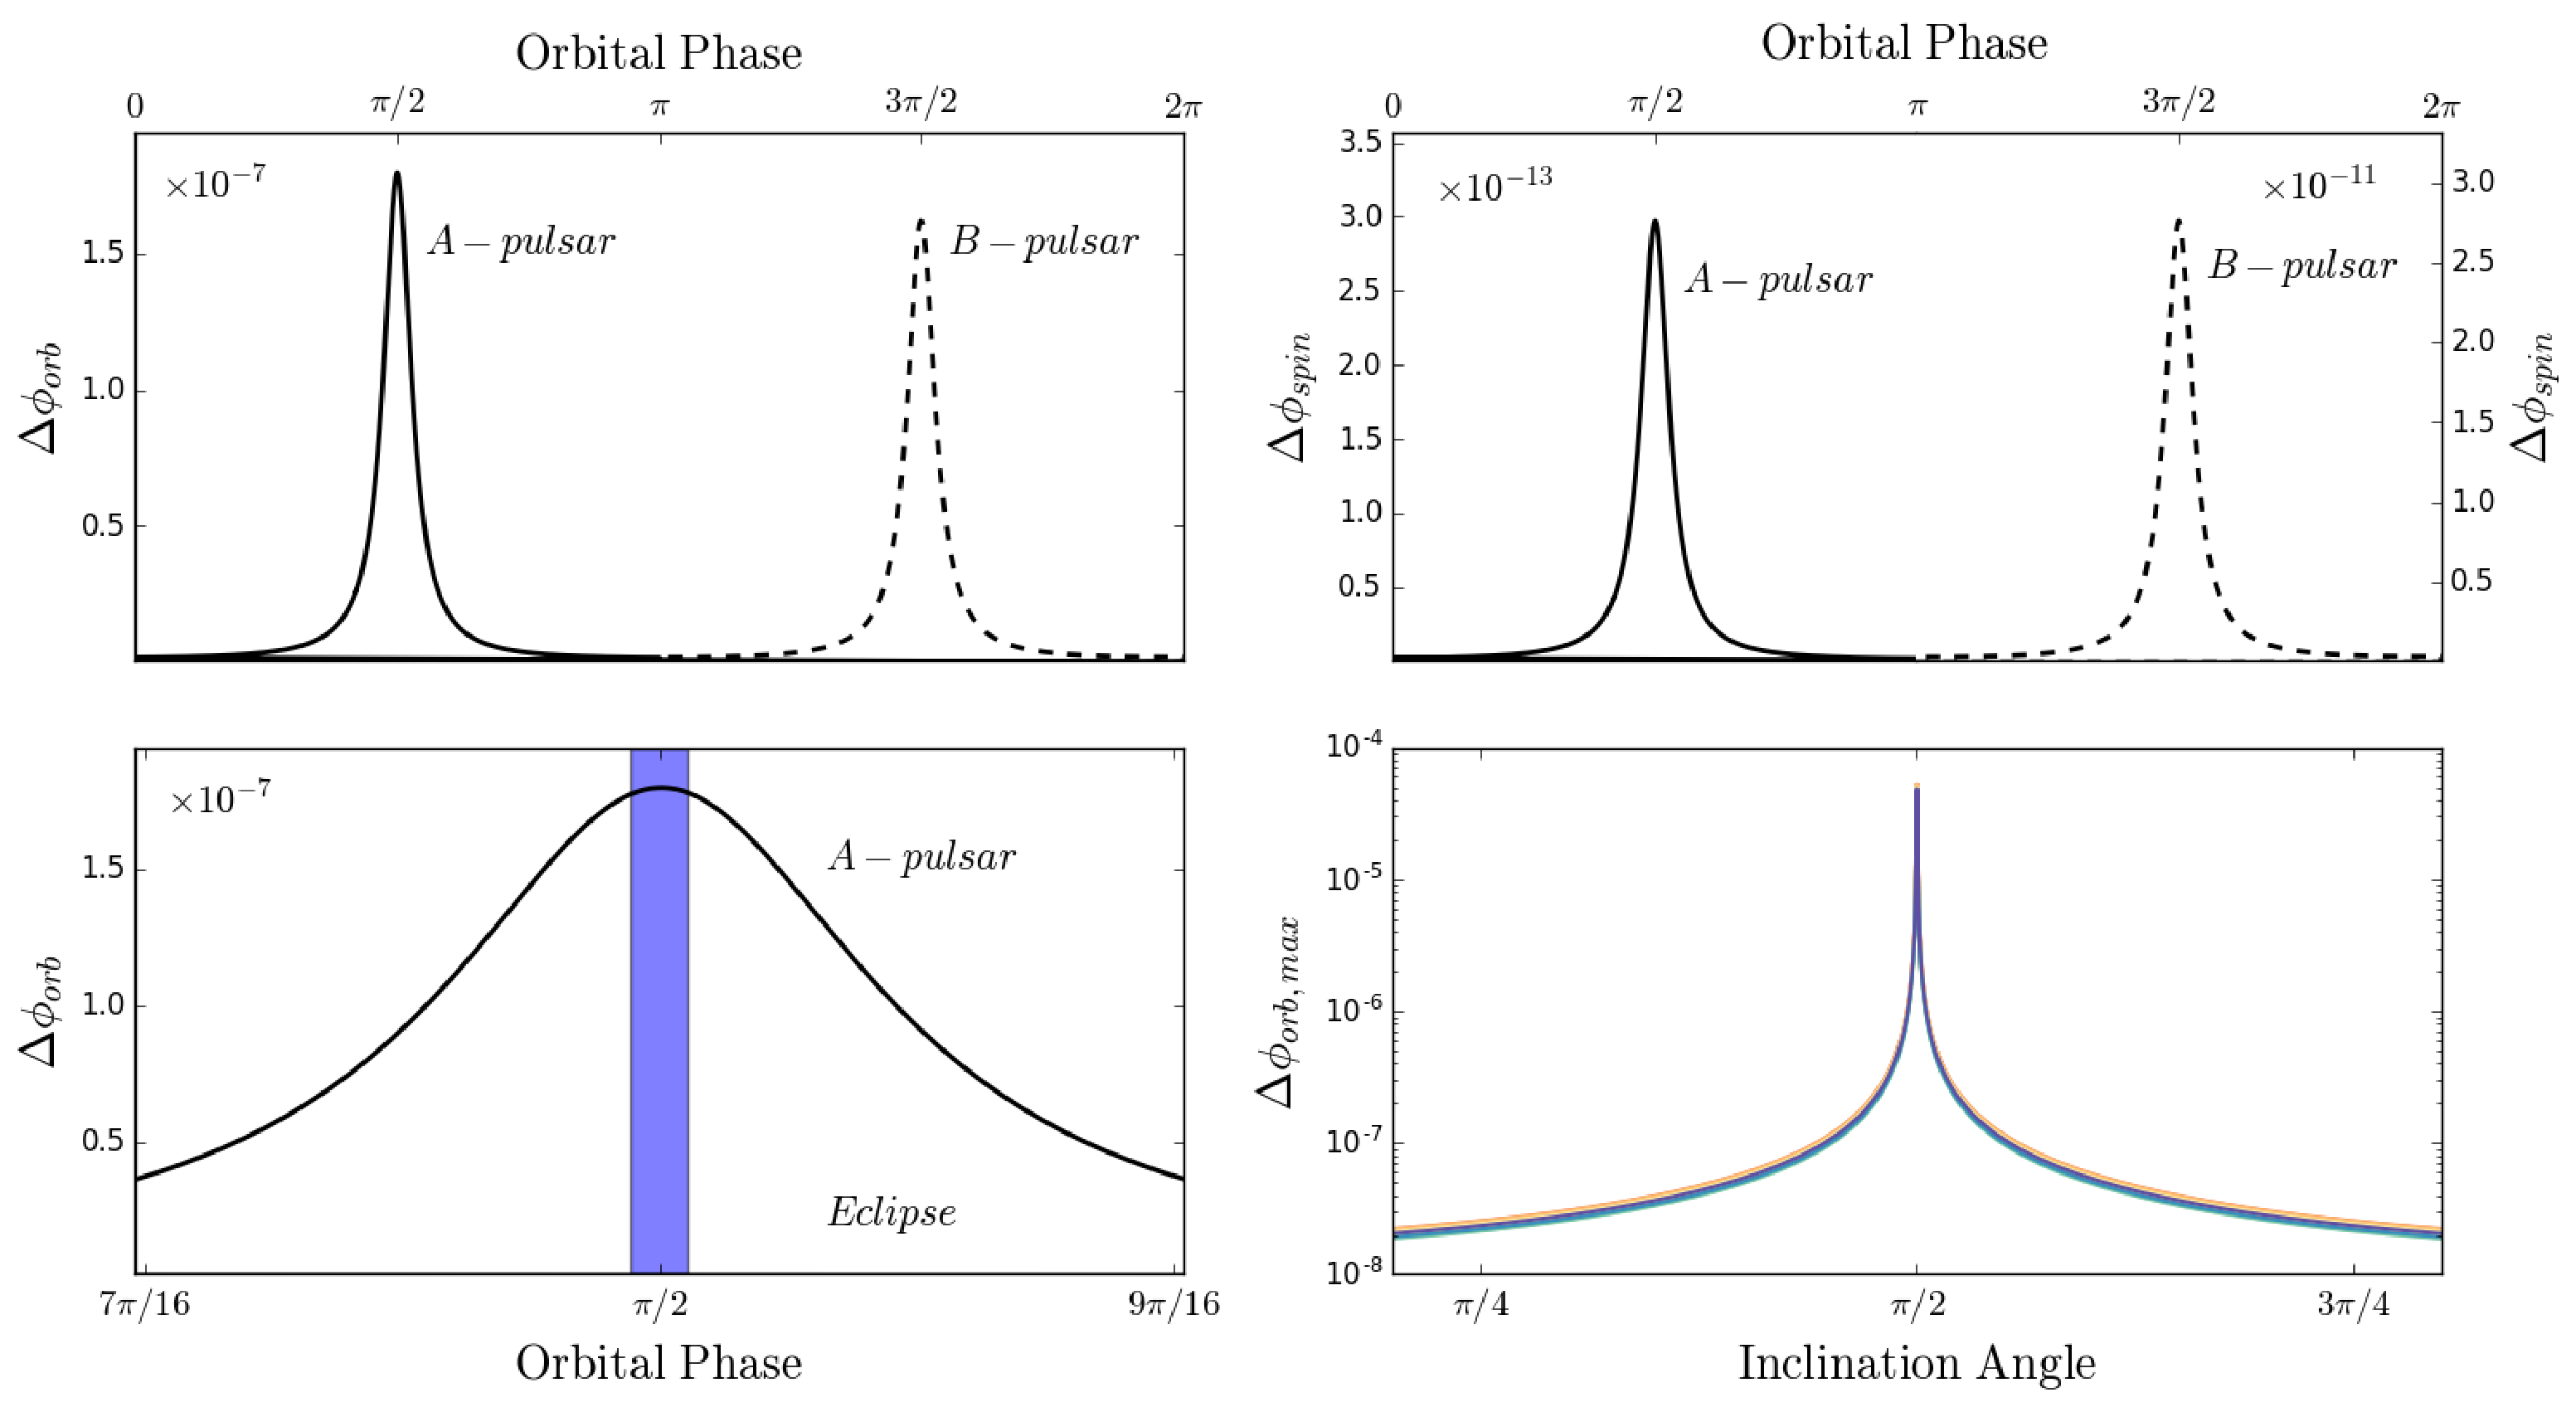
\includegraphics[width=\textwidth]{rotang.eps}
\caption{\label{fig:rotang}
The rotation angle of binary pulsar PSR J0737-3039.  }
\end{figure}







\section{Example: Double Pulsar}
\label{sec-prediction}

\subsection{Estimation}

Before we put in the actual number of the binary pulsar, let us first give a rough estimation on the maximal rotation we can get from a nearly edge-on binary neutron star system.
We take the radius of the lens neutron star to be $30km$.
If it is a slow pulsar, we take the spin period to be about $1s$.
Recall that the Schwarzschild radius of the sun is roughly $3km$, we first estimate the spin contribution in Eq.~(\ref{eq-spin}) as
\begin{equation}
S_x \sim 3km \times \frac{30km/1s}{c} \times 30km \sim 10^4 m^2~.
\end{equation}
We have used both $c$ and $G$ to make this quantity to have the unit of length$^2$, which makes it easier to calculate the unitless $\Delta\phi$.
Similarly, assume the binary orbit is $10^9 m$, velocity is about $0.1\%$ speed of light, and the orbital tilt is $2$ degree, the orbital contribution is roughly
\begin{equation}
J_x \sim 0.1\% \times 3km \times 10^9 m \times\left( \frac{4\pi}{360} \right) \sim 10^7 m^2~.
\end{equation}
In this case, the spin contribution is negligible.

If the lens is a recycled (fast) neutron star, then the period would be $\sim 1ms$, and its spin angular momentum is increased by a factor of $100$.
It will still only be $10\%$ of the orbital contribution.

The maximal rotation angle is roughly
\begin{equation}
\Delta\phi \sim 4 \frac{10^7 m^2}{\left[10^9m\times\left(\frac{4\pi}{360}\right)\right]^2}
\end{equation}

{\bf XXX:} Xin, please improve my number to be closer to the actual values.

\subsection{Prediction}

\section{Known Disagreement/Confusions}

\begin{itemize}
\item Kopeikin and Mashhoon \cite{KopMas01} agrees with the orbital angular momentum contribution, Eq.~(\ref{eq-gen}), but disagrees with the spin contribution, Eq.~(\ref{eq-spin}).
\item The previous estimation by Ruggiero and Tartaglia \cite{RugTar06} cited an equation from \cite{Ser04} which was clearly given as ``sub-leading correction''. It is suppressed by two factors of $M$ instead of one.
\end{itemize}


\bibliography{all_active}


\end{document}
